\documentclass[10pt]{article}
\usepackage{../local}


\newcommand{\classcode}{Physics 105}
\newcommand{\classname}{Analytic Mechanics}
\renewcommand{\maketitle}{%
\hrule height4pt
\large{Eric Du \hfill \classcode}
\newline
\large{HW 02} \Large{\hfill \classname \hfill} \large{\today}
\hrule height4pt \vskip .7em
\normalsize
}
\linespread{1.1}
\begin{document}
    \maketitle
    \section*{Collaborators}

    I worked with \textbf{Andrew Binder, Adarsh Iyer} and \textbf{Aren Martinian} to complete this assignment.

    \section*{Problem 1 - A Driven Oscillator}
    An oscillator of mass $m$, spring constant $k$ and damping coefficient $b$ is subject to a time-dependent driving force: 
    \[ F(t) = A\cos(\omega t) + B\cos(2\omega t)\]

    \begin{enumerate}[(a)]
        \item Find the long term behavior $x(t)$, the oscillator's position.

        \begin{solution}
            The long term behavior of the oscillator is given by $x_p(t)$, which we saw in class to have solutions of the form: 
            \[ x(t) = A_1 \cos(\omega t - \delta_1) + A_2\cos(\omega t - \delta_2)\]
            where we also have the definitions that 
            \[ A_1 = \frac{C}{\left[ (\omega_0^2 - \omega^2)^2 + 4\omega^2 \beta^2\right]}, \phantom{aa} A_2 = \frac{D}{\left[(\omega_0^2 - 4\omega^2)^2 + 16\omega^2 \beta^2\right]}\] 
            and 
            \[ \delta_1 = \tan^{-1}\left( \frac{2\beta \omega}{\omega_0^2 - \omega^2}\right) \phantom{aaaaaaa} \delta_2 = \tan^{-1} \left( \frac{4\beta \omega}{\omega_0^2 - 4\omega^2}\right)\] 
            And so therefore we write
            \[ x(t) = A_1 \cos(\omega t - \delta_1) + A_2 \cos (\omega t - \delta_2)\] 
            using $A_1, A_2, \delta_1, \delta_2$ as defined above. 
        \end{solution}
        \item Now suppose that $(b/2m)^2 < k/m$, so that the oscillator is underdamped. Given initial conditions $x(0) = 0$ and $\dot x(0) = v$, explain how to obtain equations that determine $x(t)$ fully for $t \ge 0$. Explain why $x(t)$ tends towards your answer in (a).
        
        \begin{solution}
            The homogeneous solution gives us the transient motion, and we know from lecture that $x_h(t)$ has the form: 
            \[ x_h(t) = e^{-\beta t}\left( C_1 e^{i\omega_1t} + C_2 e^{-i\omega_1t}\right)\] 
            where $\omega_1 = \sqrt{\omega_0^2 - \beta^2}$. Equivalently, we acn also rewrite this as: 
            \[ x_h(t) = Ae^{-\beta t} \cos(\omega_1t - \delta)\] 
            From here, then we can combine this with the particular solution we found above: 
            \[ x(t) = Ae^{-\beta t} \cos(\omega_1t - \delta) + A_1 \cos(\omega t - \delta _1) + A_2\cos(\omega t - \delta_2)\]
            Then, we can impose the initial conditions that $x(0) = 0$ and $x'(0) = v$ in order to solve for the coefficients $A$ and $\delta$. Unfortunately we cannot do this analytically, but this is what we should do. The solution tends towards the answer in part (a) since the transient motion $x_h(t)$ dies off over time due to the $e^{-\beta t}$ term, leaving only $x_p(t)$ remaining.
        \end{solution}
    \end{enumerate}

    \pagebreak

    \section*{Problem 2 - A Sum from Perseval's Theorem}

    In this problem you'll use Fourier series to deduce the sum

    \[ \sum_{n = 1}^\infty \frac{1}{n^4} = \frac{\pi^4}{90}\] 

    To do so, consider the function $f$ defined on $[-\pi, \pi]$ by $f(t) = t^2$. 

    \begin{enumerate}[(a)]
        \item Draw the graph of $f$. 

        \begin{solution}
            The graph of $f$ looks like the following:
            \begin{center}
                \begin{tikzpicture}[domain=-3.14:3.14, samples=100, yscale=0.5]
                    \draw[thick, stealth-stealth](-4, 0) -- (4, 0);
                    \draw[thick, stealth-stealth](0, -1) -- (0, 10);
                    \draw[color=blue] plot (\x, {\x* \x}) node[right] {$f(t) = t^2$};
                    \draw[dotted] (3.14, 0) node[below] {$\pi$}-- (3.14, 9.85);
                    \draw[dotted] (-3.14, 0)node[below] {$-\pi$} -- (-3.14, 9.85);
                \end{tikzpicture}
            \end{center}
        \end{solution}
        \item Calculate the Fourier coefficients of $f$. What is the Fourier series in terms of trigonometric functions?
        
        \begin{solution}
            From Fourier's theorem, we know that the function $f$ can be written as: 
            \[ f(t) = \frac{1}{2} a_0 + \sum_{n= 1}^\infty a_n \cos(nt)\]
            $a_0$ is relatively easy to calculate. We compute: 
            \[ a_0 = \frac{1}{2\pi}\int_{-\pi}^\pi t^2 dt = \frac{\pi^2}{3}\] 
            Now onto the $a_n$ terms.
            \[ a_n = \frac{2}{\tau} \int_{-\tau/2}^{\tau/2} t^2 \cos (nt) dt = \frac{1}{\pi} \int_{-\pi}^\pi t^2 \cos(nt) dt\]
            This integral can be solved via integration by parts twice. In order to save my wrists from typing, I'm going to skip the algebra. After the dust settles, we get:
            \[ a_n = \frac{4}{n^2}(-1)^n\]  
            And so therefore we can conclude that 
            \[ f(t) = \frac{\pi^2}{6} + \sum_{n = 1}^\infty \frac{4}{n^2} (-1)^n \cos(nt)\] 
        \end{solution}
        \item Use Parseval's theorem to find the value for the given sum. 
        
        \begin{solution}
            Parseval's theorem says:
            \[ \mean{f^2} = \mean{t^4} = |a_0|^2 + \frac 12 \sum_{n = 1}^\infty |a_n|^2\]
            First we compute $\mean{t^4}$ as we would compute it for any other interval: 
            \begin{align*}
                \mean{t^4} &= \frac{1}{2\pi}\int_{-\pi}^{\pi} t^4 dt \\
                &= \frac{\pi^4}{5}
            \end{align*}
            Now we compute the other side: 
            \begin{align*}
                |a_0|^2 + \frac 12 \sum_{n = 1}^\infty |a_n|^2 &= \frac{\pi^4}{9} + \frac 12 \sum_{n = 1}^\infty \left(\frac{4}{n^2}\right)^2\\
                &= \frac{\pi^4}{9} + 8 \sum_{n = 1}^\infty \frac{1}{n^2}
            \end{align*}
            And now we can make the two equations equal each other: 
            \begin{align*}
                \frac{\pi^4}{5} = \frac{\pi^4}{9} + 8 \sum_{n = 1}^\infty \frac{1}{n^2}\\
                \frac{4\pi^4}{45} = 8 \sum_{n = 1}^\infty \frac{1}{n^2}\\
                \therefore \sum_{n = 1}^\infty \frac{1}{n^2} = \frac{\pi^4}{90}
            \end{align*}
        \end{solution}
    \end{enumerate}

    \pagebreak

    \section*{Problem 3 - Snell's Law} 

    Fermat's principle says that the travel time of a ray of light moving from point $A$ to point $B$ is stationary. 

    \begin{center}
        \begin{tikzpicture}[decoration={markings, mark=at position 0.5 with {\arrow{stealth}}}, scale=1.5
            ]
            \draw[thick, -stealth] (-2, 0) -- (2, 0) node[above, scale=0.75] {$x$};
            \draw[thick, postaction={decorate}] (-1.6, 0.5) node[left, scale=0.75] {$P_1$} -- (0, 0);
            \draw[thick, postaction=decorate] (0, 0) -- (1.4, -1) node[below, scale=0.75] {$P_2$};
            \filldraw (1.4, -1) circle (0.03cm);
            \filldraw (-1.6, 0.5) circle (0.03cm);
            \draw[densely dashed] (-1.6, 0) node[below, scale=0.75] {$O$} -- (-1.6, 0.5);
            \draw[densely dashed] (1.4, 0) -- (1.4, -1);
            \draw[densely dashed] (0, 0.8) -- (0, -0.8);
            \draw (0, 0.4) arc (90:163:0.4);
            \draw (-0.3, 0.35) node[above,scale=0.75]{$\theta_1$};
            \draw (0, -0.4) arc(270:324:0.4);
            \draw (0.3, -0.4) node[below, scale=0.75] {$\theta_2$};
            \draw[-stealth] (-0.3, -0.3) -- (0, 0);
            \draw (-0.25, -0.25) node[below left, scale=0.75] {$Q$};
        \end{tikzpicture}
    \end{center}

    The ray of light is emitted at $P_1$, in a medium with index of refraction $n_1$. It travels through this medium until it hits a boundary at $y = 0$, after which it propagates through a medium with index of refraction $n_2$ until it arrives at $P_2$. Using Fermat's principle, derive Snell's law, which states that 
    \[ n_1 \sin \theta_1 = n_2 \sin \theta_2\] 
    It will be useful to know that light travels at speed $v = c/n$ in a medium with index of refraction $n$. 

    \begin{solution}
        We know that the time of travel can be written as: 
        \[ T = \int_{P_1}^{P_2} \frac{n(x, y)}{c} ds\] 
        Then, since we are going through two mediums, we can write: 
        \[ T = \frac{n_1}{c} \int_{P_1}^Q ds + \frac{n_2}{c} \int_Q^{P_2} ds\] 
        Here we do two things. First, let $P_1 = (x_1, y_1)$, $Q = (x, 0)$ and $P_2 = (x_2, y_2)$. Then, we compute the integral $\int ds$. From the textbook, we know that for a constant index $n$ (which is the case along path $PQ_1$ and $QP_2$), that the shortest path is a straight line. Therefore, if we write $P_1 = (x_1, y_1)$, $Q = (x, 0)$ and $P_2 = (x_2, y_2)$, then we have:
        \[ T = n_1 \sqrt{(x - x_1)^2 + y_1^2} + n_2 \sqrt{(x_2 - x)^2 + y_2^2}\] 
        Now we aim to find the location of $x$ where the time of travel is minimized, so thus we are trying to find $\dv{T}{x} = 0$. Therefore, 
        \begin{align*}
            \dv{T}{x} = 0 &= \frac{n_1}{c}\frac{1}{2\sqrt{(x - x_1)^2 + y_1^2}} \cdot 2(x - x_1) + \frac{n_2}{c}\frac{1}{2\sqrt{(x_2 - x)^2 + y_2^2}} \cdot 2(x_2 - x) (-1)\\
            &= \frac{n_1}{c} \underbrace{\frac{x - x_1}{\sqrt{(x - x_1)^2 + y_1^2}}}_{\sin \theta_1} - \frac{n_2}{c} \underbrace{\frac{x_2 - x}{\sqrt{(x_2 - x)^2 + y_2^2}}}_{\sin \theta_2}
        \end{align*}
        And so therefore we get
        \[ n_1 \sin \theta_1 = n_2 \sin \theta_2\] 
    \end{solution}

    \pagebreak

    \section*{Problem 4 - Double Atwood Machine}

    The figure below shows a double Atwood machine. The center pulley is free to move verticaly and has mass $M$. The (ideal, massless) string connecting the three masses shown is weightless. Masses $m_1$ and $m_2$ hang on the left and right respectively of the fixed pulleys. The acceleration of gravity is $g$. All three pulleys are frictionless, so that the string slides freely over them. 

    (Credit to Andrew Binder for this Ti\textit kZ diagram)
    \begin{center}
        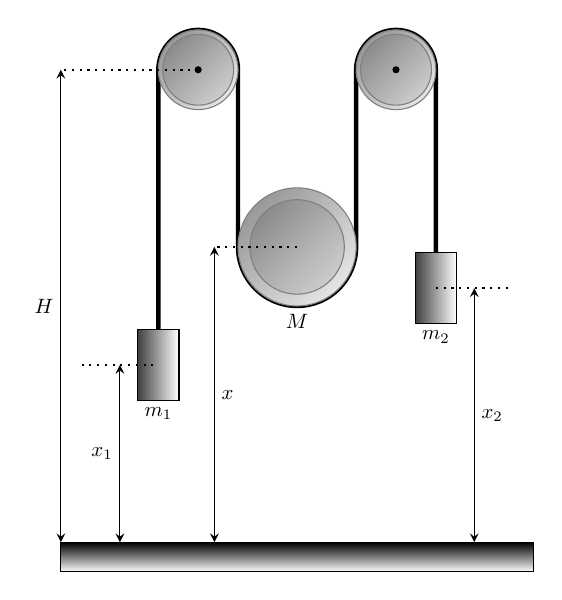
\begin{tikzpicture}[scale=1.5]
            \draw[shading=axis, top color=black, bottom color=white, shading angle=0, anchor=north] (-2,-0.5) -- (2,-0.5) -- (2,-0.75) -- (-2,-0.75) -- cycle;
            \draw[ultra thick] (-1.175,1.3) -- (-1.175,3.5) to[bend left=45] (-0.8375,3.8375) to[bend left=45] (-0.5,3.5) -- (-0.5,2) to[bend right=45] (0,1.5) node[anchor=north,scale=0.75] {$M$} to[bend right=45] (0.5,2) -- (0.5,3.5) to[bend left=45] (0.8375,3.8375) to[bend left=45] (1.175,3.5) -- (1.175,1.95);
            \draw[gray, shading=axis, left color=gray!80, right color=gray!20!white, shading angle=45, anchor=north] (0,2) circle (0.5cm);
            \draw[gray, shading=axis, left color=gray!90, right color=gray!40!white, shading angle=45, anchor=north] (0,2) circle (0.4cm);
            \draw[shading=axis, left color=gray!150, right color=white, shading angle=90, anchor=north] (1,1.95) -- (1.35,1.95) -- (1.35,1.35) -- (1,1.35) node[midway,below,scale=0.75] {$m_2$} -- cycle;
            \draw[shading=axis, left color=gray!150, right color=white, shading angle=90, anchor=north] (-1.35,1.3) -- (-1,1.3) -- (-1,0.7) -- (-1.35,0.7) node[midway,below,scale=0.75] {$m_1$} -- cycle;
            \draw[gray, shading=axis, left color=gray!80, right color=gray!20!white, shading angle=45, anchor=north] (0.8375,3.5) circle (0.3375cm);
            \draw[gray, shading=axis, left color=gray!90, right color=gray!40!white, shading angle=45, anchor=north] (0.8375,3.5) circle (0.3cm);
            \filldraw[black] (0.8375,3.5) circle (0.025cm);
            \draw[gray, shading=axis, left color=gray!80, right color=gray!20!white, shading angle=45, anchor=north] (-0.8375,3.5) circle (0.3375cm);
            \draw[gray, shading=axis, left color=gray!90, right color=gray!40!white, shading angle=45, anchor=north] (-0.8375,3.5) circle (0.3cm);
            \filldraw[black] (-0.8375,3.5) circle (0.025cm);
            \draw[thick, dotted] (-1.825,1) -- (-1.175,1);
            \draw[stealth-stealth] (-1.5,-0.5) -- (-1.5,1) node[midway,left,scale=0.75] {$x_1$};
            \draw[thick, dotted] (1.175,1.65) -- (1.825,1.65);
            \draw[stealth-stealth] (1.5,-0.5) -- (1.5,1.65) node[midway,right,scale=0.75] {$x_2$};
            \draw[thick,dotted] (0,2) -- (-0.7,2);
            \draw[stealth-stealth] (-0.7,-0.5) -- (-0.7,2) node[midway,right,scale=0.75] {$x$};
            \draw[stealth-stealth] (-2, -0.5) -- (-2, 3.5) node[midway,left, scale=0.75]{$H$};
            \draw[thick, dotted] (-0.8375, 3.5) -- (-2, 3.5);
        \end{tikzpicture}
    \end{center}

    \begin{enumerate}[(a)]
        \item By considering carefully the forces acting on each mass and pulley, and the constraint imposed by the string's length being fixed, show that the equations of motion are:
        \[ \begin{cases}
            \left( m_1 + \frac{M}{4}\right) \ddot x_1 + \frac{M}{4} \ddot x_2 = g\left( \frac M2 - m_1\right), \\ 
            \frac M4 \ddot x_1 + \left( m_2 + \frac M4 \right) \ddot x_2 = g\left( \frac {M}{2} - m_2\right)
        \end{cases}\] 

        \begin{solution}
            First, we write down the equations of motion: 
            \begin{align*}
                m_1 \ddot x_1 &= -m_1g + T_1\\
                m_2 \ddot x_2 &= -m_2g + T_2\\
                M\ddot x &= -Mg + T_1 + T_2
            \end{align*}
            Now becuase the rope is frictionless, we know that $T_1 = T_2$. Thus, we now have the equations: 
            \begin{align}
                m_1 \ddot x_1 &= -m_1g + T\\
                m_2 \ddot x_2 &= -m_2g + T\\
                M\ddot x &= -Mg + 2T
            \end{align}
            Now, let $H$ be defined as in the diagram above. We can now find the total length of the rope (excluding the $\pi r$ terms denoting the length of the rope on the pulleys themselves): 
            \[ (H - x_1) + (H - x_2) + 2(H - x) = L\] 
            And since the length of the rope doesn't change in time, we have $\dv{L}{t} = 0$, so therefore: 
            \begin{align*}
                \dot x_1 + \dot x_2 + 2\dot x &= 0\\
                \ddot x_1 + \ddot x_2 + 2 \ddot x &= 0\\
                \therefore \ddot x =-\left( \frac{\ddot x_1 + \ddot x_2}{2}\right)
            \end{align*}
            Now, we can subtract twice the first equation by the third to get
            \begin{align*}
                2m_1 \ddot x_1 - M\ddot x &= -2m_1g + Mg
            \end{align*}
            And so now we can apply the constraint and solve: 
            \begin{align*}
                2m_1 \ddot x_1 + M\left( \frac{\ddot x_1 + \ddot x_2}{2}\right) &= -2m_1g + Mg\\
                m_1 \ddot x_1 + M\left( \frac{\ddot x_1 + \ddot x_2}{4}\right) &= -m_1g + \frac{M}{2}g\\
                \therefore \ddot x_1 \left(m_1 + \frac M4\right) + \ddot x_2 \frac M4 &= g\left( \frac M2 - m_1\right)
            \end{align*}
            The exact same algebra exists for the other equation:
            \begin{align*}
                2m_2 \ddot x_2 + M\left( \frac{\ddot x_1 + \ddot x_2}{2}\right) &= -2m_2g + Mg\\
                m_2 \ddot x_2 + M\left( \frac{\ddot x_1 + \ddot x_2}{4}\right) &= -m_2g + \frac{M}{2}g\\
                \therefore \ddot x_2 \left( m_2 + \frac{M}{4}\right) + \ddot x_1 \frac{M}{4} &= g\left(\frac{M}{2} - m_2\right)
            \end{align*}
        \end{solution}
        \item Solve this problem again, this time by writing down the Lagrangian, and finding the equations of motion. 

        \begin{solution}
            We have the kinetic and potential energies:
            \begin{align*}
                T &= \frac 12 m_1\dot x_1^2 + \frac 12 m_2 \dot x_2^2 + \frac 12 M \dot x^2\\
                U &= mgx_1 + mgx_2 + mgx
            \end{align*}
            Therefore the Lagrangian is: 
            \[ \mathcal{L} = T - U = \frac 12 m_1 \dot x_1^2 + \frac 12 \dot x_2^2 + \frac 12 M \dot x^2 - m_1gx_1 - m_1gx_2 - Mgx\] 
            Here we can now use the constraint equation $2\dot x + \dot x_1 + \dot x_2 = 0$ in order to get: 
            \[ \mathcal L = \frac12 m_1 \dot x_1^2 + \frac 12 \dot x_2^2 + \frac 12 M \left(\frac{\dot x_1^2 + 2\dot x_1 \dot x_2 + \dot x_2^2}{2}\right)^2 - m_1gx_1 - m_2gx_2 - Mg\left(\frac{x_1 + x_2}{2}\right)\] 
            This is a lagrangian with two coordinates, $x_1$ and $x_2$, and so therefore we can do them separately. Writing down the Euler-Lagrange equation for $x_1$: 
            \[ \pdv{\mathcal L}{x_1} = -m_1g + \frac 12 Mg = \dv{t}\left( m_1 \dot x_1 + \frac{2}{8} \dot x_1 M + \frac{2\dot x_2}{8} M\right)\]
            We have three terms on the rightmost side here because in the expansion of $\dot x_1^2 + 2\dot x_1 \dot x_2 + \dot x_2^2$ we have two terms containing $\dot x_1$. Now, we can rearrange: 
            \begin{align*}
                -m_1g + \frac 12 Mg &= m_1 \ddot x_1 + \frac 14 M \ddot x_1 + \frac 14 M \ddot x_2\\
                \therefore \ddot x_1\left(m_1 + \frac M4\right) + \frac M4 \ddot x_2 &= g\left( \frac M2 - m_1\right)
            \end{align*} 
            The exact same algebra (in fact, the equations are symmetric for $x_1$ and $x_2$) follows for $x_2$: 
            \begin{align*}
                \pdv{\mathcal L}{x_2} = -m_2g + \frac 12 Mg &= \dv{t}\left(m_2 \dot x_2 + \frac{2}{8} \dot x_2M + \frac{2\dot x_1}{8}M\right)\\
                -m_2g + \frac 12 Mg &= m_2 \ddot x_2 + \frac 14 M \ddot x_2 + \frac 14 \ddot x_1\\
                \therefore  \frac M4 \ddot x_1 + \ddot x_2 \left( m_2 + \frac M4 \right) &= g\left( \frac {M}{2} - m_2\right)
            \end{align*}
        \end{solution}
    \end{enumerate}


    \pagebreak

    \section*{Problem 5}

    Consider the Lagrangian of some physical system $L(q, \dot q, t)$, where $q$ is a generalized coordinate and $t$ is time. The action is given by $S[L] = \int L dt$. Suppose we add a function to the Lagrangian $f(q, \dot q, t)$. Show that if $f$ is a total time derivative, then the equations of motion are unchanged. Try to think of other modifications to the Lagrangian that preserve the equations of motion.

    \begin{solution}
        If $f$ is a total time derivative, then it means we can write: 
        \[ \dv{f}{t} = \pdv{f}{q}\dot q(t) + \pdv{f}{t}\] 
        Then, we can now add this onto $\mathcal L$ to get $\mathcal L' = \mathcal L + f$, and then now we can write down the Euler-Lagrange equations: 
        \[ \pdv{\mathcal L}{q} - \dv{t} \pdv{\mathcal L}{\dot q} + \pdv{q}\dv{f}{t} - \dv{t} \pdv{f}{\dot q} = 0\] 
        We know that the first two terms equal zero since they are part of the ``original'' Lagrangian. Therefore we only need to look at the last two terms:
        \[ \pdv{q} \left( \dv{f}{t}\right) - \dv{t}\pdv{\dot q}\left( \dv{f}{t}\right)\]
        And we can substitute the first relation into here to get: 
        \begin{align*}
            \pdv{q}\left(\dv{f}{t}\right) - \dv{t}\left[\pdv{\dot q}\left(\pdv{f}{q}\dot q + \pdv{f}{t}\right)\right] &= \pdv{q} \left( \dv{f}{t}\right) - \dv{t}\left[\pdv{\dot q} \dv{f}{q} \dot q + \pdv{\dot q} \dv{f}{t}\right]\\
            &= \pdv{q}\dv{f}{t} - \dv t\left[ \pdv{\dot q} \dv{f}{q} \dot q + \pdv{f}{\dot q} + \pdv{\dot q} \dv{f}{t}\right]\\
            &= \pdv{q}\dv{f}{t}  - \dv{t} \pdv{f}{q} = 0
        \end{align*}
        where in the last step we've used the relation that $\pdv{q} \dv{f}{t} = \dv{t} \pdv{f}{q}$ - namely the fact that we can switch the order in which we take the derivatives. Since they equal zero, then it means that we've verified our equations of motion, and so therefore the equations of motion are preserved.

        In general, we can see that any modification that alters our coordinate axes (in other words, transforming $q(t)$ into some arbitrary $q'(t)$) should preserve the Lagrangian, since the motion of a system should not be dependent on the way we look at it. These transformations should also not alter the Lagrangian at all, and so the equation of motion remains the same.
    \end{solution}

\end{document}